\documentclass[12pt]{article}
\usepackage{amsmath}
\usepackage{amssymb}
\usepackage{physics}
\usepackage{enumitem}
\usepackage{ctex} 
\usepackage{graphicx}
\usepackage{float}
\begin{document}

\title{中国原子能科学研究院2023年博士研究生入学考试\\普通物理试题(整理版)}
\author{}
\date{}
\maketitle

\section*{试题部分}
\begin{enumerate}[label=\arabic*.]
    \item 判断平衡态(4分)\\
    金属杆与沸水和冰接触,各点温度不随时间变化,是否处于平衡态?为什么?
    
    \item 单缝衍射分析(8分)\\
    讨论单缝夫琅禾费衍射实验中:
    \begin{enumerate}
        \item 缝宽减半时衍射图样变化
        \item 入射光波长增大时条纹变化
        \item 单缝平移时条纹变化
        \item 入射光倾斜入射时的变化
        \item 使用白光光源时的现象
    \end{enumerate}

    
    \item 电场强度计算(8分)\\
    半径$R$的均匀带电球体(电荷量$Q$),挖去半径$r$的小球后,求球心处电场强度$\vec{E}$及$P$、$Q$、$R$点电势。
    
    \item 干涉条纹分析(8分)\\
    双缝干涉实验中,当$\lambda=490$nm,$d=490$μm时,求干涉条纹开始模糊的级数。
    
    \item 综合计算(12分)
    \begin{enumerate}
        \item 正三角形顶点处有电荷$+q$、$+q$、$-q$,求中心点$P$、$Q$、$R$的电势和电场强度
        \item 锂原子基态电子激发相关计算
        \item 气体绝热过程分析:已知状态方程$P(V-b)=RT$,内能$U=CT+U_0$,求准静态绝热过程方程
    \end{enumerate}
\end{enumerate}

\section*{完整解答}
\begin{enumerate}
    \item \textbf{平衡态判断} \\
    金属杆\textbf{不处于平衡态}。根据热力学平衡条件:
    \begin{itemize}
        \item 虽然宏观温度分布稳定($\pdv{T}{t}=0$)
        \item 但存在温度梯度(沸水端$T_1$,冰端$T_2$,$T_1 > T_2$)
        \item 持续存在热传导过程($\dd{Q} = -\kappa A \dv{T}{x} \dd{t} \neq 0$)
    \end{itemize}
    结论:属于稳态而非平衡态。
    
    \item \textbf{衍射图样分析}
    \begin{enumerate}
        \item 缝宽$a$减半:中央明纹宽度$\Delta x = 2\lambda f/a$ → 宽度加倍
        \item 波长$\lambda$增大:$\Delta x \propto \lambda$ → 条纹间距增大
        \item 单缝平移:衍射图样不变(夫琅禾费衍射的平移不变性)
        \item 倾斜入射角$\theta_0$:衍射斑整体平移$\Delta x = f \sin\theta_0$
        \item 白光入射:产生彩色光谱,中央明纹仍为白色
    \end{enumerate}
          \begin{itemize}
    \item (1) 所有明纹变宽,条纹间距增大
    \item (2)--(4)见图片
    \begin{figure}[H]
        \centering
        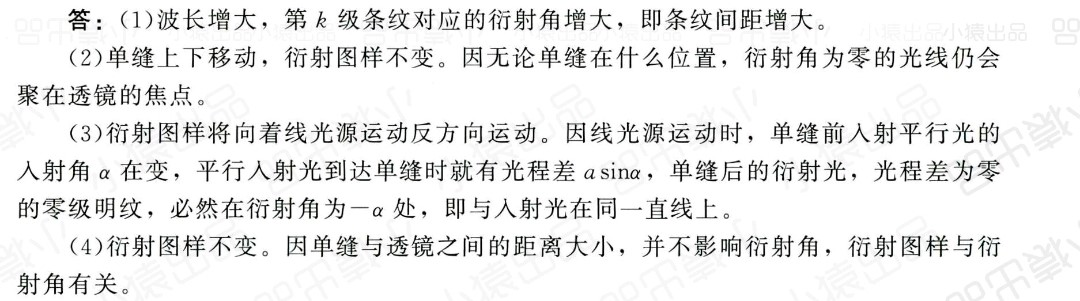
\includegraphics[width=1.3\linewidth]{Screenshot_20250416_215216.jpg}
    \end{figure}
  \end{itemize}
  
    \item \textbf{电场强度计算} \\
    应用叠加原理和高斯定理:
    \begin{align*}
        \rho &= \frac{Q}{\frac{4}{3}\pi R^3} \\
        Q_{\text{挖}} &= \rho \cdot \frac{4}{3}\pi r^3 = Q\left(\frac{r}{R}\right)^3 \\
        \vec{E} &= \frac{1}{4\pi\epsilon_0}\left[ \frac{Q}{R^3}\vec{r} - \frac{Q(r/R)^3}{r^3}\vec{r} \right] \\
        &= \frac{Q}{4\pi\epsilon_0 R^3}\left(1 - \frac{r^3}{R^3}\right)\vec{r}
    \end{align*}
    电势计算需分段积分,球心处$U=\frac{Q}{4\pi\epsilon_0 R}\left(1-\frac{r^2}{R^2}\right)$
    
    \item \textbf{干涉条纹模糊} \\
    最大干涉级条件:
    \begin{gather*}
        2d \sin\theta = k\lambda \\
        \sin\theta_{\text{max}} = 1 \Rightarrow k_{\text{max}} = \frac{2d}{\lambda} = \frac{2\times490}{0.49} = 2000 \\
        \text{模糊条件:} \Delta k = 1 \Rightarrow \text{从}k=3\text{级开始模糊}
    \end{gather*}
    
    \item \textbf{综合计算}
    \begin{enumerate}
        \item 电势计算(边长$a$):
        \begin{align*}
            r &= \frac{\sqrt{3}}{3}a \\
            U_P &= \frac{1}{4\pi\epsilon_0}\left(\frac{q}{r} + \frac{q}{r} - \frac{q}{r}\right) = \frac{q}{4\pi\epsilon_0 r} \\
            \vec{E}_P &= \frac{\sqrt{3}q}{4\pi\epsilon_0 a^2}(\hat{i} + \hat{j})
        \end{align*}
        
        \item 锂原子基态(略,需具体参数)
        
        \item 绝热过程方程推导:
        \begin{gather*}
            \dd{U} = C \dd{T} = -P \dd{V} \\
            \frac{C}{R}(P \dd{V} + (V-b)\dd{P}) = -P \dd{V} \\
            \gamma = 1 + \frac{R}{C} \\
            \Rightarrow P(V-b)^\gamma = \text{const.}
        \end{gather*}
    \end{enumerate}
\end{enumerate}

\end{document}